\chapter{我要出去逛逛}



% \pagecolor{gray}
\AddToShipoutPicture*{\put(-50,-80){
\includegraphics[scale=1.2]{./res/jpegs/mouse-reading.jpeg}}} % Image background
{\linespread{1.5}\fontsize{18}{18}\selectfont
\vspace*{2cm}
小老鼠坐在沙发上看了半天书,眼睛有点发干,腿脚有点发麻。
长时间坐着对身体不太好吧。他想出去逛逛。不知道外面天气怎么样?\par
}
\ClearShipoutPicture

\newpage
\AddToShipoutPicture*{\put(-50,-80){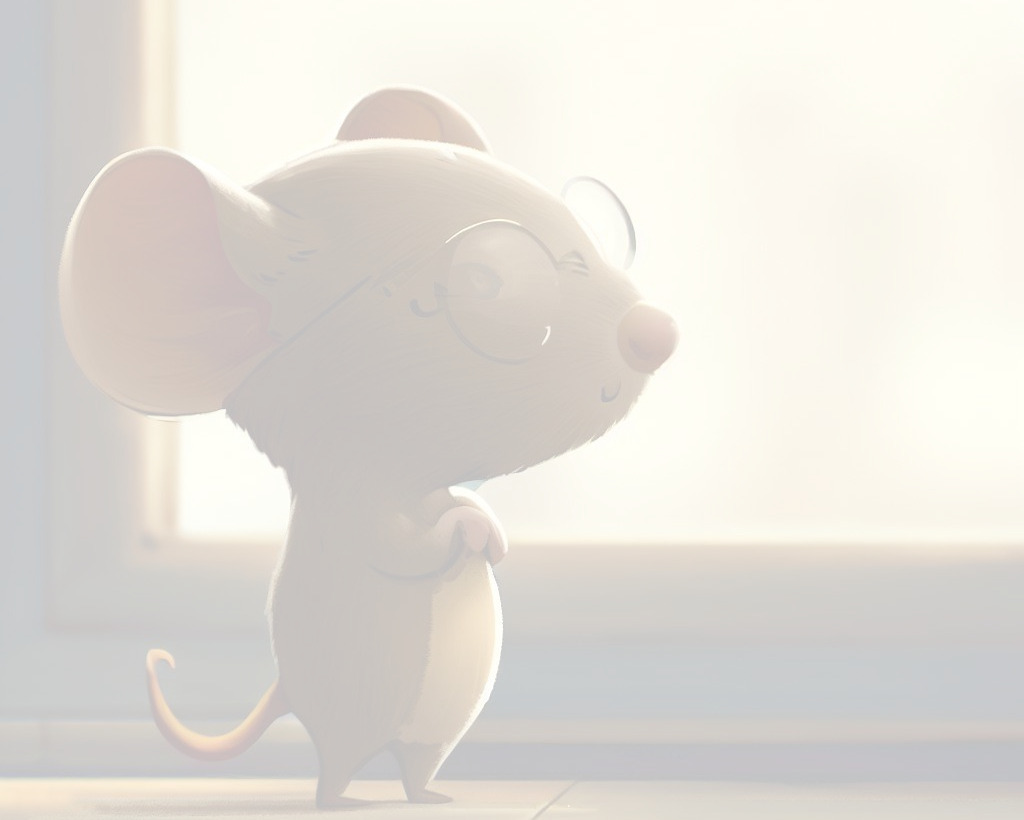
\includegraphics[scale=1.2]{./res/jpegs/mouse-window.jpeg}}} % Image background
{\linespread{1.5}\fontsize{18}{18}\selectfont
\vspace*{2cm}
他走到窗户旁边。 \par
}
\vspace*{15pt}
\begin{adjustbox}{angle=18}
{\linespread{1.1}\fontsize{28}{28}\selectfont
踢踢腿
\par}
\end{adjustbox}
\begin{adjustbox}{angle=18}
{\linespread{1.1}\fontsize{28}{28}\selectfont
伸伸懒腰
\par}
\end{adjustbox}
{\linespread{1.1}\fontsize{28}{28}\selectfont
看看外面的大树和青草。
\par}
\vspace*{5pt}
{\linespread{1.5}\fontsize{18}{18}\selectfont
哇! 外面阳光明媚, 天气好好啊!
\par}
\ClearShipoutPicture





\chapter{找到一个翘翘板}

\AddToShipoutPicture*{\put(-50,-80){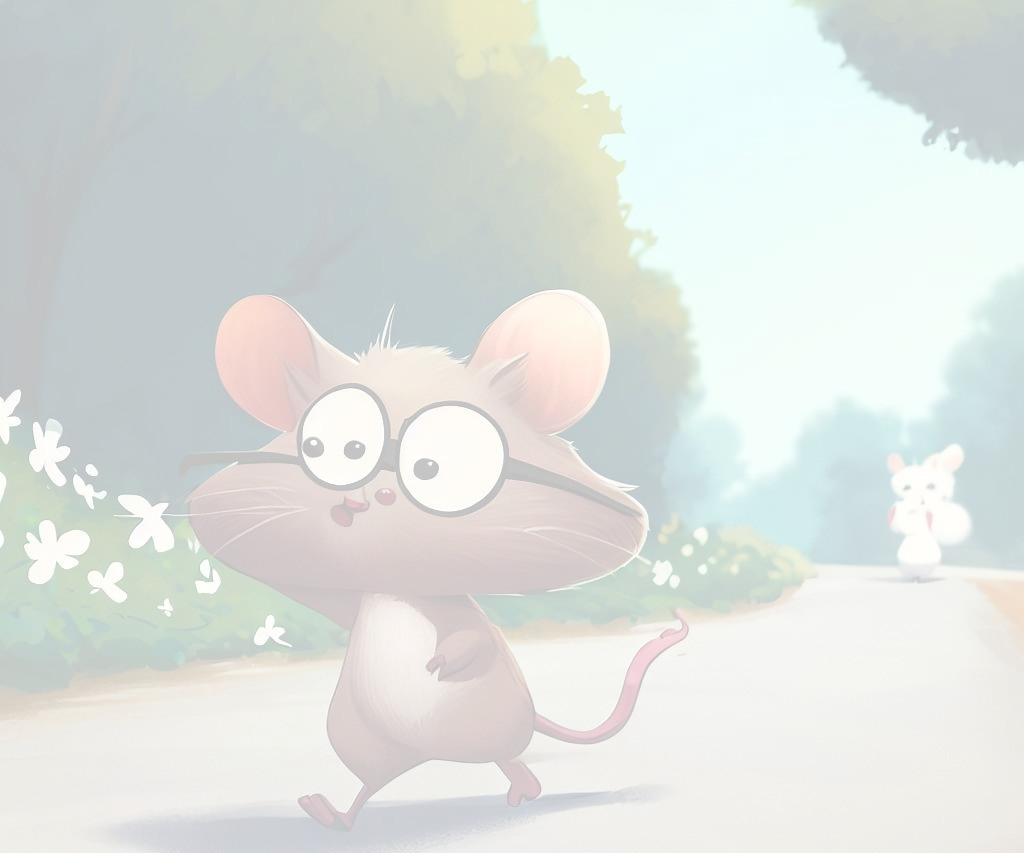
\includegraphics[scale=1.2]{./res/jpegs/mouse-out.jpeg}}} % Image background
\vspace*{15pt}
{\linespread{1.1}\fontsize{48}{48}\selectfont
走起!
\par}
\vspace*{15pt}
{\linespread{1.5}\fontsize{18}{18}\selectfont
出去玩啦!
呼吸一下新鲜空气。
\par}
{\linespread{1.5}\fontsize{18}{18}\selectfont
咦,这是谁远远地跟在小老鼠后面?
\par}
\ClearShipoutPicture



\newpage
\AddToShipoutPicture*{\put(-50,-80){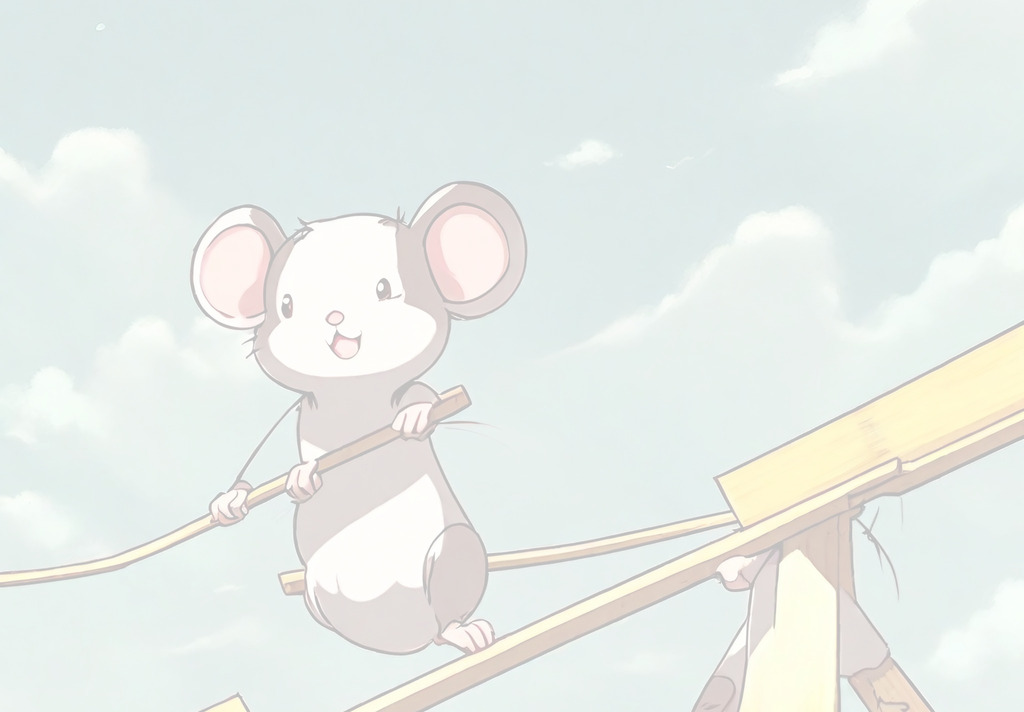
\includegraphics[scale=4.5]{./res/jpegs/mouse-on-seesaw.jpeg}}} % Image background
\vspace*{15pt}
{\linespread{1.1}\fontsize{48}{48}\selectfont
到公园啦!
\par}
\vspace*{15pt}
{\linespread{1.5}\fontsize{18}{18}\selectfont
看看公园里面有什么好玩的?\par
\par}
{\linespread{1.5}\fontsize{18}{18}\selectfont
哈哈,找到一个翘翘板!\par
我坐上去啦!
\par}
\ClearShipoutPicture

\chapter{我怎么飞起来了?}

\AddToShipoutPicture*{\put(-50,-80){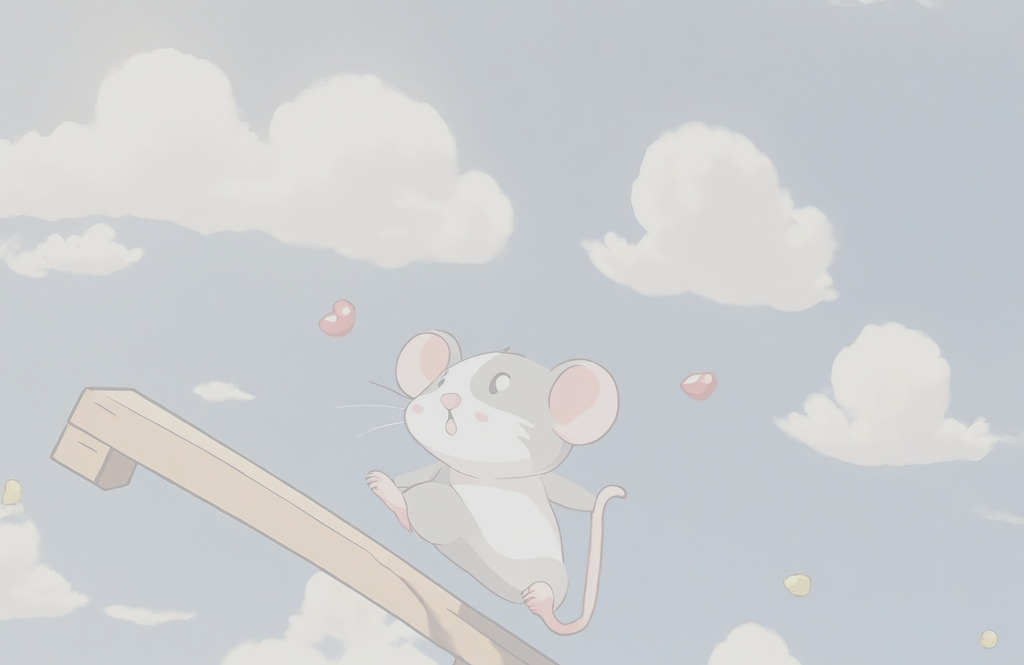
\includegraphics[scale=4.5]{./res/jpegs/mouse-in-sky.jpeg}}} % Image background
\par
\vspace*{15pt}
{\linespread{1.5}\fontsize{18}{18}\selectfont
刚才不是还坐在翘翘板上吗?
\par}
{\linespread{1.5}\fontsize{18}{18}\selectfont
怎么现在到了半空啦?\par
小老鼠不明白发生了什么。
\par}
\ClearShipoutPicture

\newpage
\AddToShipoutPicture*{\put(-50,-80){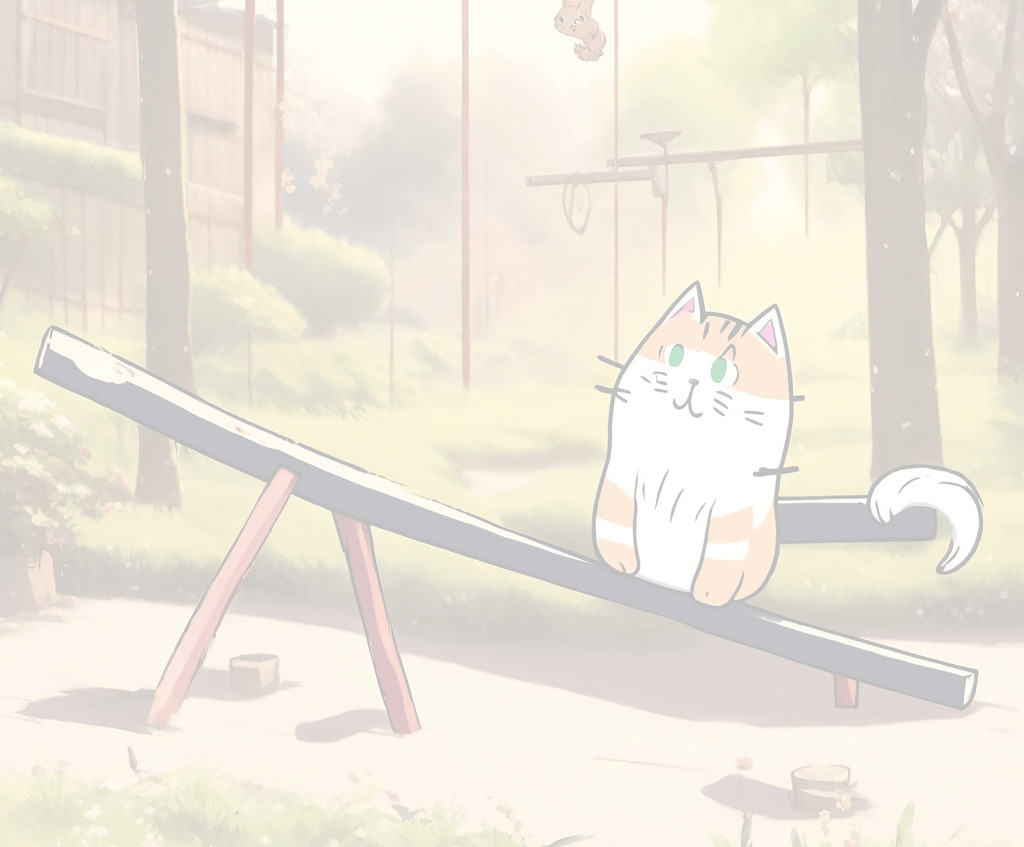
\includegraphics[scale=4.2]{./res/jpegs/cat-on-seesaw-fs8.jpeg}}} % Image background
\vspace*{15pt}
{\linespread{1.5}\fontsize{18}{18}\selectfont
它低头一看,\par
原来是小猫跳到翘翘板上,\par
自己这一边突然被撬起来了!\par
小猫很得意。\par
小老鼠,你太小了。\par
我一坐下来,\par
你就飞到天上去了!\par
\par
\par}
\ClearShipoutPicture

\newpage
\AddToShipoutPicture*{\put(-50,-80){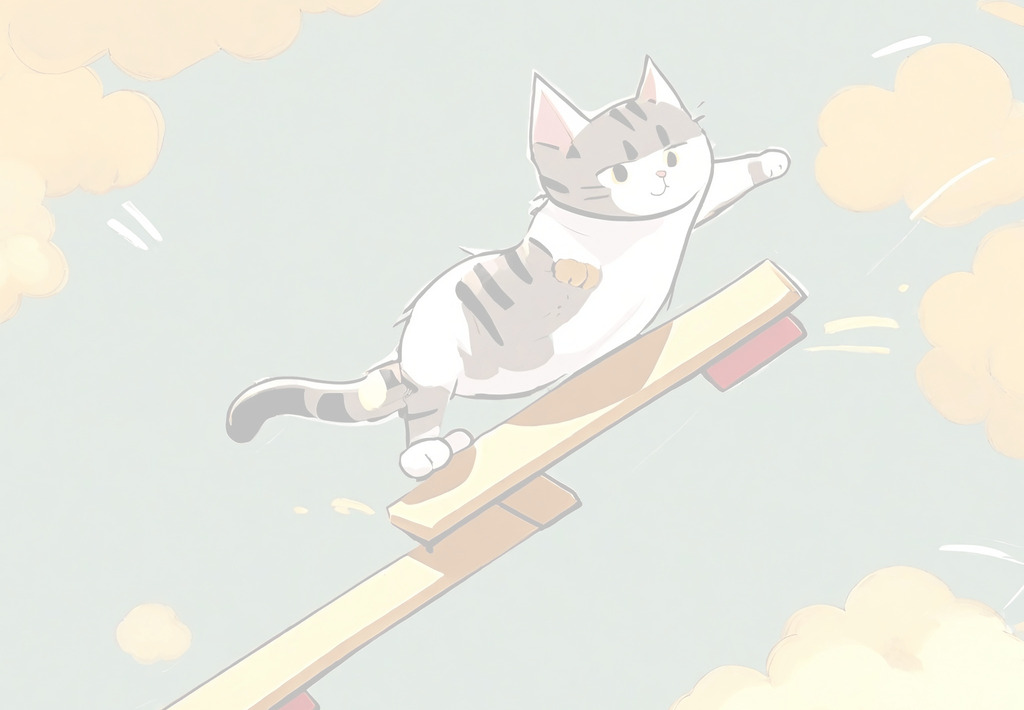
\includegraphics[scale=4.2]{./res/jpegs/cat-in-sky-fs8.jpeg}}} % Image background
\vspace*{15pt}
{\linespread{1.5}\fontsize{18}{18}\selectfont
\par
可正当它哈哈笑的时候,\par
它也飞起来了!\par
这是怎么回事?\par
刚才不是还坐在翘翘板上吗?\par
怎么现在到了半空啦?\par
\par
\par}
\ClearShipoutPicture


\newpage
\AddToShipoutPicture*{\put(-0,-0){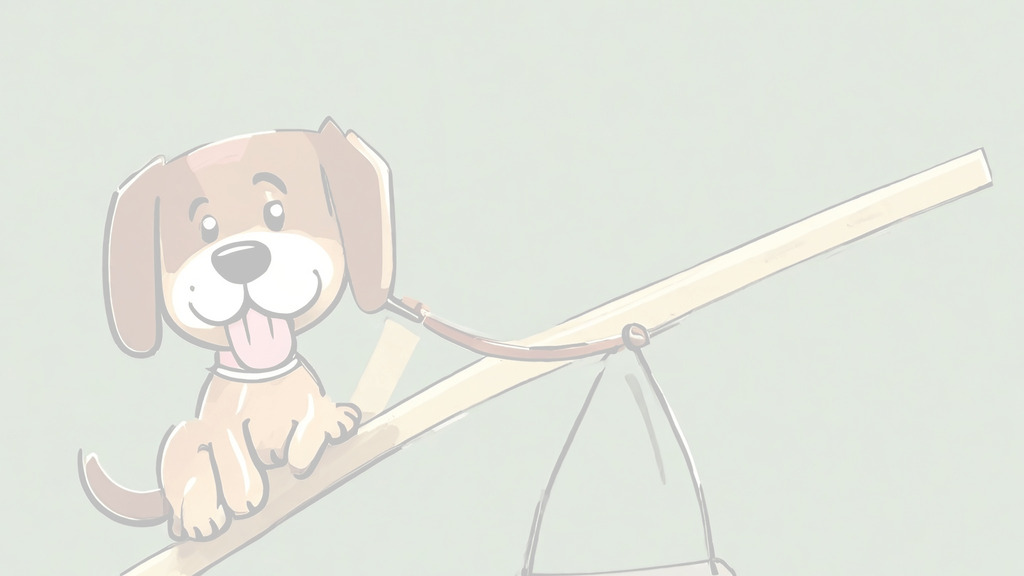
\includegraphics[scale=4.9]{./res/jpegs/dog-on-seesaw-fs8.jpeg}}} % Image background
\vspace*{15pt}
{\linespread{1.5}\fontsize{18}{18}\selectfont
\par
它低头一看,\par
原来是小狗跳到翘翘板上,\par
自己这一边突然被撬起来了!\par
小狗很得意。\par
小猫,你太小了。\par
我一坐下来,\par
你就飞到天上去了!\par
\par
\par}
\ClearShipoutPicture



\newpage
\AddToShipoutPicture*{\put(-0,-0){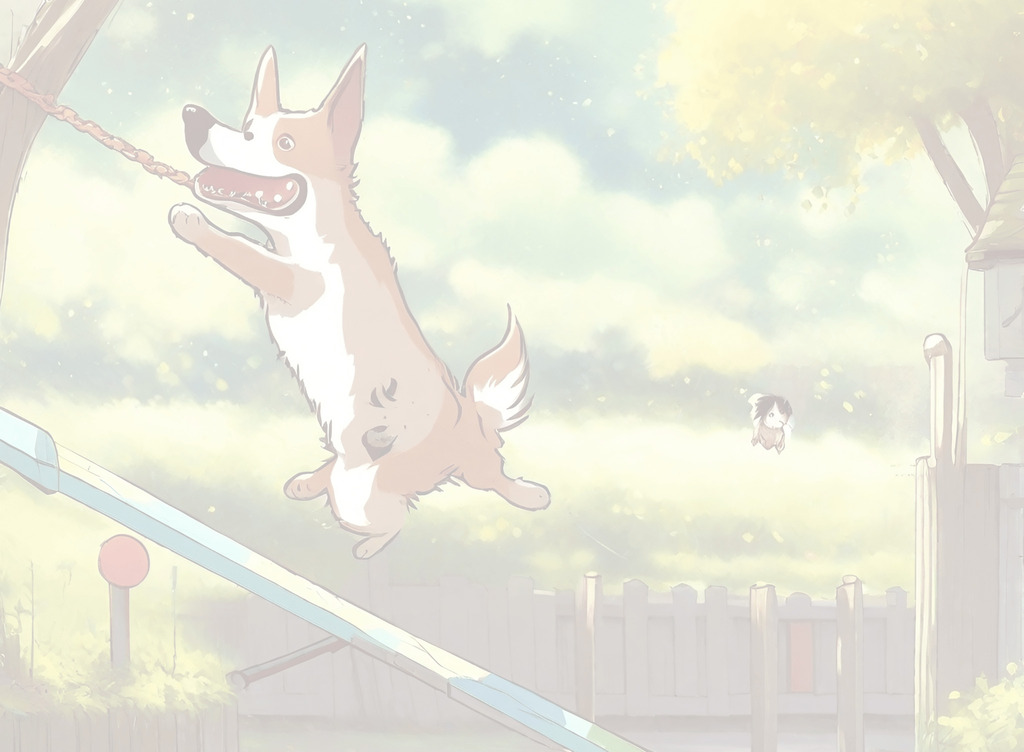
\includegraphics[scale=4.2]{./res/jpegs/dog-in-sky-fs8.jpeg}}} % Image background
\vspace*{15pt}
{\linespread{1.5}\fontsize{18}{18}\selectfont
\par
可正当它哈哈笑的时候,\par
它也飞起来了!\par
这是怎么回事?\par
刚才不是还坐在翘翘板上吗?\par
怎么现在到了半空啦?\par
\par
\par}
\ClearShipoutPicture



\newpage
\AddToShipoutPicture*{\put(-50,-80){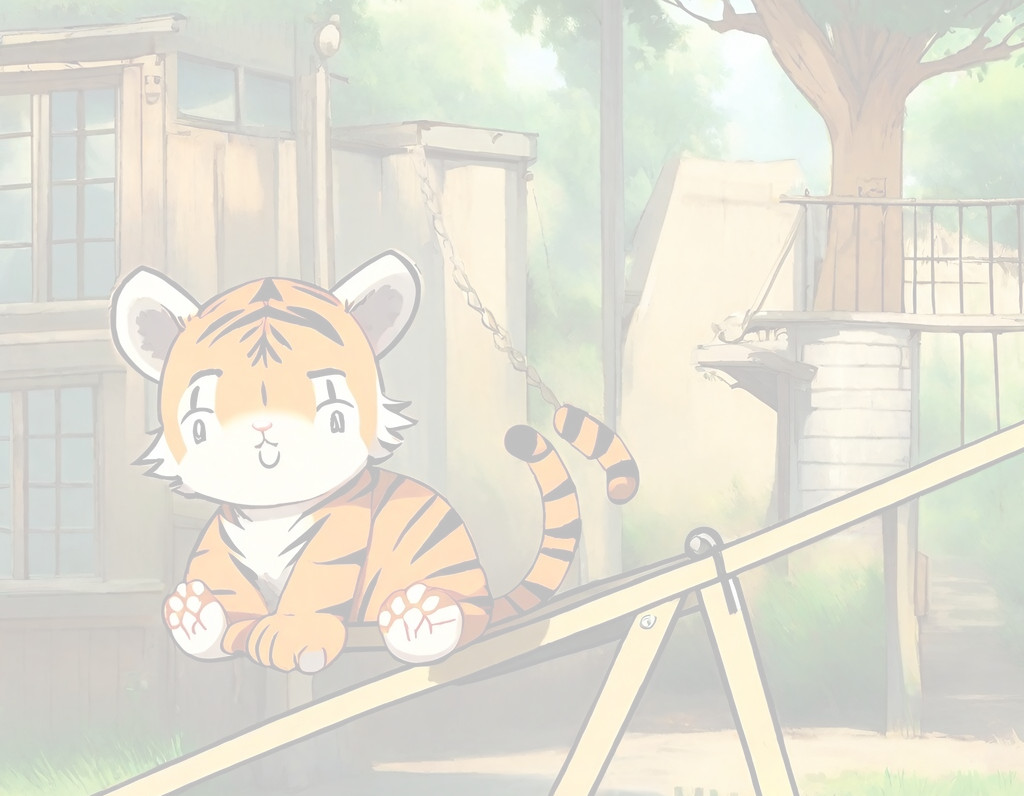
\includegraphics[scale=1.2]{./res/jpegs/tiger-on-seesaw.jpeg}}} % Image background
\vspace*{15pt}
{\linespread{1.5}\fontsize{18}{18}\selectfont
\par
它低头一看,\par
原来是小老虎跳到翘翘板上,\par
自己这一边突然被撬起来了!\par
小虎很得意。\par
小狗,你太小了。\par
我一坐下来,\par
你就飞到天上去了!\par
\par
\par}
\ClearShipoutPicture



\newpage
\AddToShipoutPicture*{\put(-50,-80){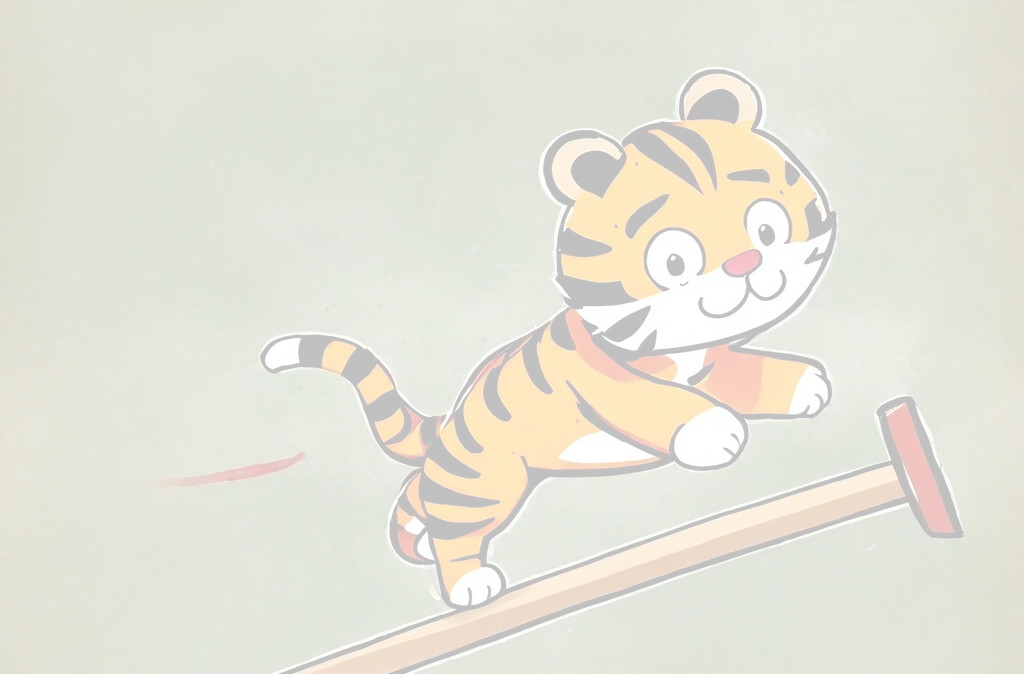
\includegraphics[scale=1.2]{./res/jpegs/tiger-in-sky.jpeg}}} % Image background
\vspace*{15pt}
{\linespread{1.5}\fontsize{18}{18}\selectfont
\par
可正当它哈哈笑的时候,\par
它也飞起来了!\par
这是怎么回事?\par
刚才不是还坐在翘翘板上吗?\par
怎么现在到了半空啦?\par
\par

\par}
\ClearShipoutPicture



\newpage
\AddToShipoutPicture*{\put(-50,-80){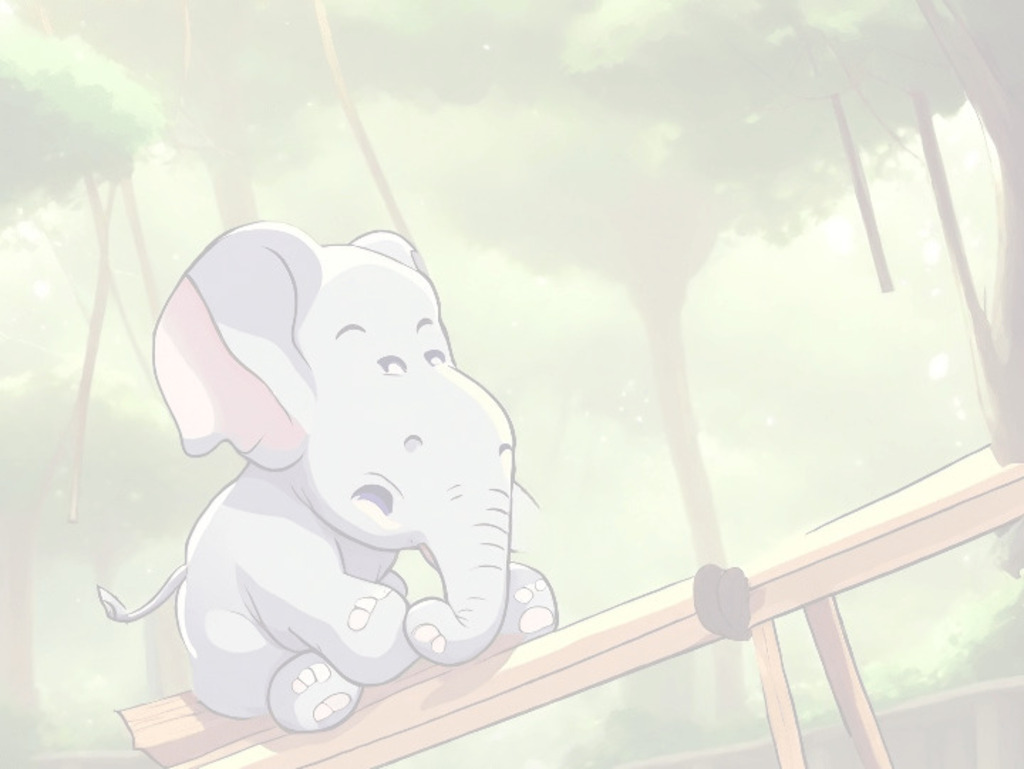
\includegraphics[scale=4.2]{./res/jpegs/elephant-on-seesaw-fs8.jpeg}}} % Image background
\vspace*{15pt}
{\linespread{1.5}\fontsize{18}{18}\selectfont
\par
它低头一看,\par
原来是大象跳到翘翘板上,\par
自己这一边突然被撬起来了!\par
大象很得意。\par
小老虎,你太小了。\par
我一坐下来,\par
你就飞到天上去了!\par
\par
\par}
% \ClearShipoutPicture



\newpage
\AddToShipoutPicture*{\put(-5,-8){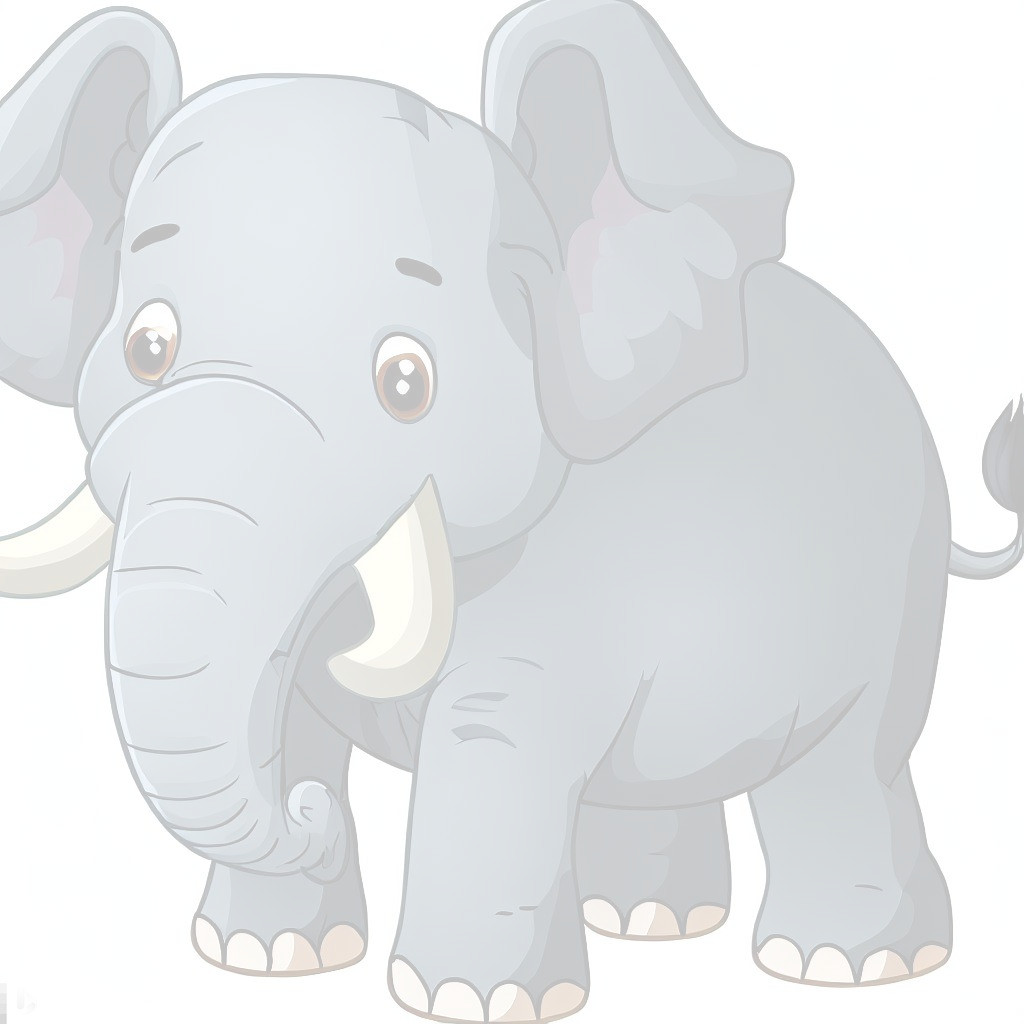
\includegraphics[scale=1.2]{./res/jpegs/elephant_huge.jpeg}}} % Image background
\vspace*{15pt}
{\linespread{1.5}\fontsize{18}{18}\selectfont
\par
大象哈哈笑着说,\par
我是陆地上最大的动物,\par
你们所有人都撬不动我!\par
\par
\par}
\ClearShipoutPicture



\newpage
\AddToShipoutPicture*{\put(-50,-80){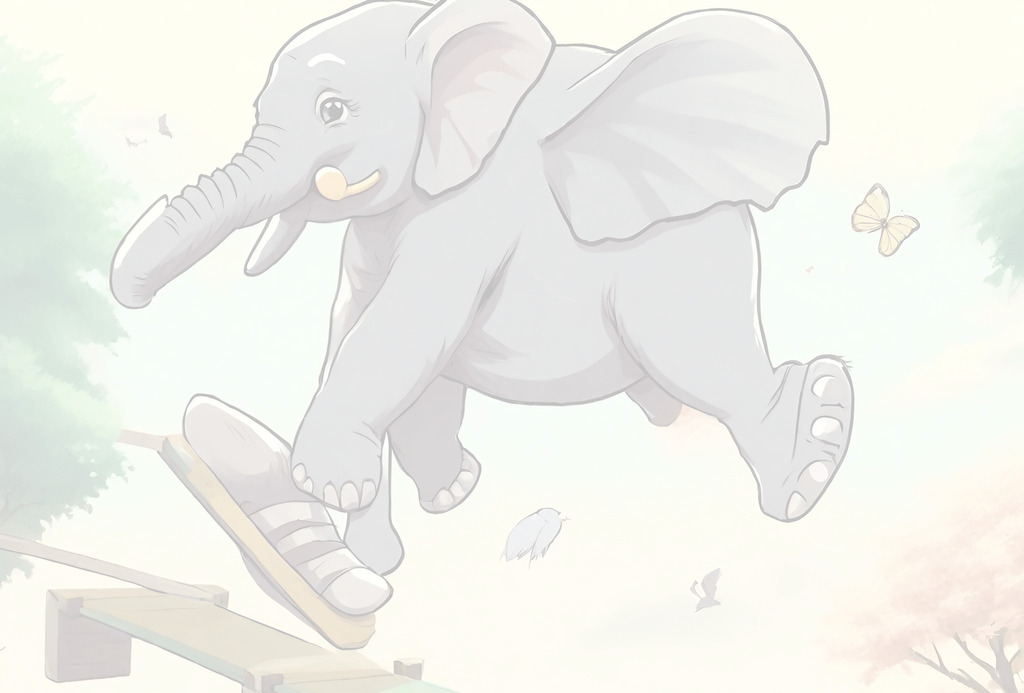
\includegraphics[scale=4.2]{./res/jpegs/elephant-in-sky-fs8.jpeg}}} % Image background
\vspace*{15pt}
{\linespread{1.5}\fontsize{18}{18}\selectfont
\par
\par
可正当它哈哈笑的时候,\par
它也飞起来了!\par
这怎么可能?\par
\par
\par}
\ClearShipoutPicture

\newpage
\AddToShipoutPicture*{\put(-150,-8){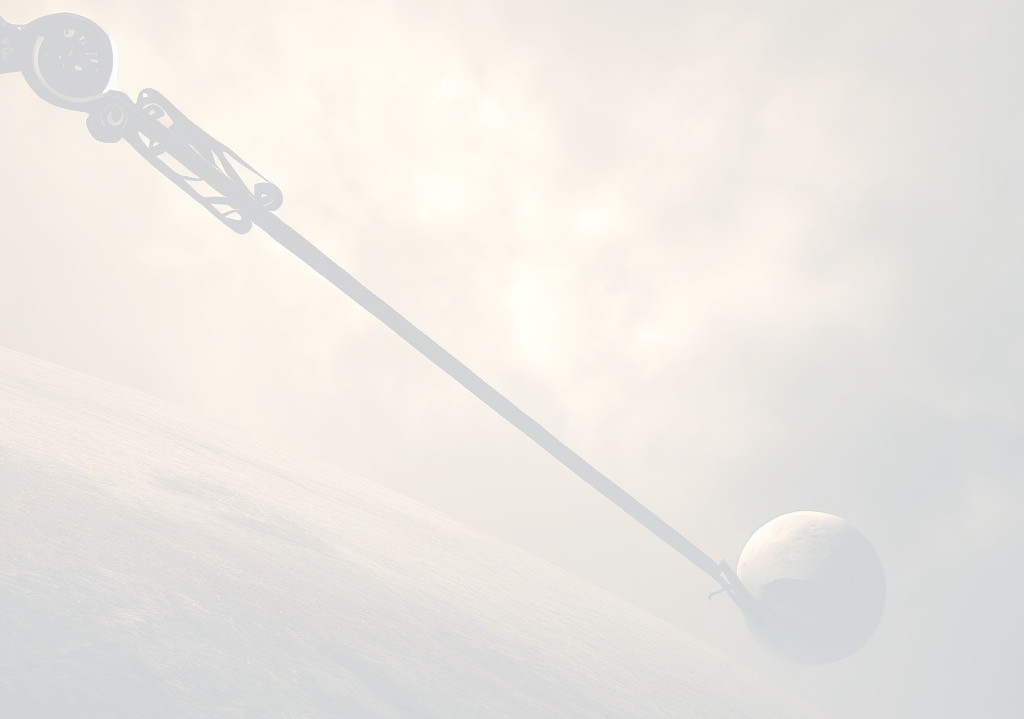
\includegraphics[scale=1.5]{./res/jpegs/earth-leverage.jpeg}}} % Image background
\vspace*{15pt}
{\linespread{1.5}\fontsize{18}{18}\selectfont
\par
\par
它低头一看,\par
原来是小动物们把翘翘板的另一边加长啦,\par
翘翘板变成了大杠杆,\par
自己这一边突然被撬起来了!\par
\par
\par}
\ClearShipoutPicture






\pagenumbering{gobble}
\newpage
\thispagestyle{empty}
\EANisbn[ISBN=978-80-7340-097-2]